\documentclass{article}

\usepackage{fancyhdr}
\usepackage{extramarks}
\usepackage{amsmath}
\usepackage{amsthm}
\usepackage{amsfonts}
\usepackage{tikz}
\usepackage[plain]{algorithm}
\usepackage{algpseudocode}
\usepackage{graphicx}
\usepackage{gensymb}
\usepackage{calc}
\usepackage[framed,numbered,autolinebreaks,useliterate]{mcode}
\usepackage{listings}

\graphicspath{{./images/}}

\usetikzlibrary{automata,positioning}

%
% Basic Document Settings
%

\topmargin=-0.45in
\evensidemargin=0in
\oddsidemargin=0in
\textwidth=6.5in
\textheight=9.0in
\headsep=0.25in

\linespread{1.1}

\pagestyle{fancy}
\lhead{\hmwkAuthorName}
\chead{\hmwkClass\ \hmwkTitle}
\rhead{\firstxmark}
\lfoot{\lastxmark}
\cfoot{\thepage}

\renewcommand\headrulewidth{0.4pt}
\renewcommand\footrulewidth{0.4pt}

\setlength\parindent{0pt}

%
% Create Problem Sections
%

\newcommand{\enterProblemHeader}[1]{
    \nobreak\extramarks{}{Problem {#1} continued on next page\ldots}\nobreak{}
    \nobreak\extramarks{{#1} (continued)}{{#1} continued on next page\ldots}\nobreak{}
}

\newcommand{\exitProblemHeader}[1]{
    \nobreak\extramarks{{#1} (continued)}{{#1} continued on next page\ldots}\nobreak{}
    % \stepcounter{#1}
    \nobreak\extramarks{{#1}}{}\nobreak{}
}

\setcounter{secnumdepth}{0}
\newcounter{partCounter}

\newcommand{\problemNumber}{0.0}

\newenvironment{homeworkProblem}[1][-1]{
    \renewcommand{\problemNumber}{{#1}}
    \section{\problemNumber}
    \setcounter{partCounter}{1}
    \enterProblemHeader{\problemNumber}
}{
    \exitProblemHeader{\problemNumber}
}

%
% Homework Details
%   - Title
%   - Class
%   - Author
%

\newcommand{\hmwkTitle}{Midterm}
\newcommand{\hmwkClass}{RBE 500}
\newcommand{\hmwkAuthorName}{\textbf{Arjan Gupta}}

%
% Title Page
%

\title{
    \vspace{2in}
    \textmd{\textbf{\hmwkClass\ \hmwkTitle}}\\
    \vspace{3in}
}

\author{\hmwkAuthorName}
\date{}

\renewcommand{\part}[1]{\textbf{\large Part \Alph{partCounter}}\stepcounter{partCounter}\\}

%
% Various Helper Commands
%

% Useful for algorithms
\newcommand{\alg}[1]{\textsc{\bfseries \footnotesize #1}}

% For derivatives
\newcommand{\deriv}[2]{\frac{\mathrm{d}}{\mathrm{d}#2} \left(#1\right)}

% For compact derivatives
\newcommand{\derivcomp}[2]{\frac{\mathrm{d}#1}{\mathrm{d}#2}}

% For partial derivatives
\newcommand{\pderiv}[2]{\frac{\partial}{\partial #2} \left(#1\right)}

% For compact partial derivatives
\newcommand{\pderivcomp}[2]{\frac{\partial #1}{\partial #2}}

% Integral dx
\newcommand{\dx}{\mathrm{d}x}

% Alias for the Solution section header
\newcommand{\solution}{\textbf{\large Solution}}

% Probability commands: Expectation, Variance, Covariance, Bias
\newcommand{\E}{\mathrm{E}}
\newcommand{\Var}{\mathrm{Var}}
\newcommand{\Cov}{\mathrm{Cov}}
\newcommand{\Bias}{\mathrm{Bias}}

\newlength\dlf% Define a new measure, dlf
\newcommand\alignedbox[2]{
% Argument #1 = before & if there were no box (lhs)
% Argument #2 = after & if there were no box (rhs)
&  % Alignment sign of the line
{
\settowidth\dlf{$\displaystyle #1$}  
    % The width of \dlf is the width of the lhs, with a displaystyle font
\addtolength\dlf{\fboxsep+\fboxrule}  
    % Add to it the distance to the box, and the width of the line of the box
\hspace{-\dlf}  
    % Move everything dlf units to the left, so that & #1 #2 is aligned under #1 & #2
\boxed{#1 #2}
    % Put a box around lhs and rhs
}
}

\begin{document}

\maketitle

\nobreak\extramarks{Problem 1}{}\nobreak{}

\pagebreak

\begin{homeworkProblem}[Problem 1]
    Derive the rotation matrix $R^1_2$ (you can leave sines and cosines as is).

    \begin{figure}[h]
        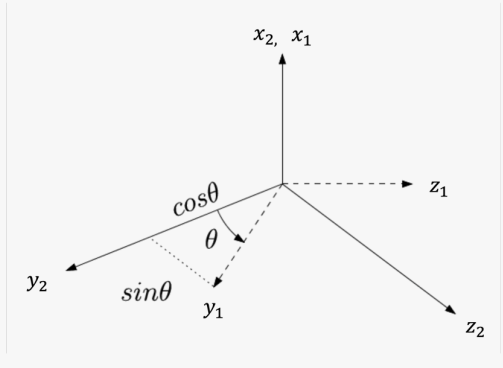
\includegraphics[scale=0.4]{q1_figure.png}
        \centering
    \end{figure}

    \subsection{Solution}

    Since the x-axis remains the same in the rotation, we know this is a basic 3D rotation matrix representing a rotation
    about the x-axis. However, using the right-hand screw rule, we see that the angle $\theta$ here is negative. So, by
    using equation 2.7 (page 43) of our main textbook, the rotation matrix is given by,

    \begin{align*}
        &R^1_2 =
        \begin{bmatrix}
            1 & 0 & 0\\
            0 & \cos(-\theta) & -\sin(-\theta)\\
            0 & \sin(-\theta) & \cos(-\theta)\\
        \end{bmatrix}\\
        \alignedbox{}{R^1_2=
        \begin{bmatrix}
            1 & 0 & 0\\
            0 & \cos\theta & \sin\theta\\
            0 & -\sin\theta & \cos\theta\\
        \end{bmatrix}}
    \end{align*}
\end{homeworkProblem}

\nobreak\extramarks{Problem 2}{}\nobreak{}

\pagebreak

\begin{homeworkProblem}[Problem 2]
    Find the coordinates of point $p$ expressed in frame 1 (i.e. $p^1$) given the following.

    \[H^2_1 = \begin{bmatrix}
        1 & 0 & 0 & -1\\
        0 & 0.9553 & 0.2955 & -0.9553\\
        0 & -0.2955 & 0.9553 & 0.2955\\
        0 & 0 & 0 & 1
    \end{bmatrix},\text{   } p^2 = \begin{bmatrix}
        2\\
        5\\
        0
    \end{bmatrix}\]

    \subsection{Solution}

    From our knowledge of homogeneous transformations, we know that

    \[P^2 = H^2_1 P^1\]

    Where
    \(P^2 = \begin{bmatrix}
        p^2\\
        1
    \end{bmatrix}\) and \(P^1 = \begin{bmatrix}
        p^1\\
        1
    \end{bmatrix}\).\\

    However, we want to find $P^1$, so we apply the inverse of H to both sides,

    \begin{align*}
        P^2 &= H^2_1 P^1\\
        {(H^2_1)}^{-1}P^2 &= P^1
    \end{align*}

    We know that \(H^2_1 = \begin{bmatrix}
        R^2_1 & d^2_1\\
        0 & 1
    \end{bmatrix}\), where \(R^2_1 = \begin{bmatrix}
        1 & 0 & 0\\
        0 & 0.9553 & 0.2955\\
        0 & -0.2955 & 0.9553
    \end{bmatrix}\) and \(d^2_1 = \begin{bmatrix}
        -1\\
        -0.9553\\
        0.2955
    \end{bmatrix}\).\\
    \vspace{0.15in}\\
    For accuracy while computing the inverse of $H^2_1$, we use equation 2.67 of the book (page 63).
    Therefore, \[{(H^2_1)}^{-1} = \begin{bmatrix}
        {(R^2_1)}^T & -{(R^2_1)}^T d^2_1\\
        0 & 1
    \end{bmatrix}\].
    We use the following MATLAB code for this computation.
    \lstinputlisting{prob2_midterm.m}
    % H2_1 = [1 0 0 -1; 0 0.9553 0.2955 -0.9553; 0 -0.2955 0.9553 0.2955; 0 0 0 1];
    % inv(H2_1)*P2

    Which gives us the answer,

    \[
        \boxed{P^1 = \begin{bmatrix}
            3.0000\\
            5.7764\\
            1.4775\\
            1.0000
        \end{bmatrix}}
    \]
\end{homeworkProblem}

\nobreak\extramarks{Problem 3}{}\nobreak{}

\pagebreak

\begin{homeworkProblem}[Problem 3]
    If \(R^0_1 = \begin{bmatrix}
        0.7071& 0& 0.7071\\
        0 & 1 & 0\\
        -0.7071& 0& 0.7071
    \end{bmatrix}\), 
    \(R^0_2 = \begin{bmatrix}
        0 & 0.866 & 0.5\\
        0 & 0.5 & -0.866\\
        -1 & 0 & 0
    \end{bmatrix}\), and 
    \(R^0_3 = \begin{bmatrix}
        0 & -1 & 0\\
        0 & 0 & 1\\
        -1 & 0 & 0
    \end{bmatrix}\), calculate $R^1_2$.

    \subsection{Solution}

    Knowing the composition law for rotational transformations, we can write

    \begin{align*}
        R^1_2 &= R^1_0 R^0_2\\
        R^1_2 &= {(R^0_1)}^T R^0_2\\
        R^1_2 &= {\begin{bmatrix}
            0.7071& 0& 0.7071\\
            0 & 1 & 0\\
            -0.7071& 0& 0.7071
        \end{bmatrix}}^T 
        \begin{bmatrix}
            0 & 0.866 & 0.5\\
            0 & 0.5 & -0.866\\
            -1 & 0 & 0
        \end{bmatrix}\\
        R^1_2 &= {\begin{bmatrix}
            0.7071& 0& -0.7071\\
            0 & 1 & 0\\
            0.7071& 0& 0.7071
        \end{bmatrix}} 
        \begin{bmatrix}
            0 & 0.866 & 0.5\\
            0 & 0.5 & -0.866\\
            -1 & 0 & 0
        \end{bmatrix}\\
    \end{align*}

    We use the following MATLAB script to compute this multiplication.
    \lstinputlisting{prob3_midterm.m}

    Therefore,
    \[
        \boxed{
            R^1_2 =
            \begin{bmatrix}
                0.7071 & 0.6123 & 0.3535\\
                0 & 0.5000 & -0.8660\\
               -0.7071 & 0.6123 & 0.3535
            \end{bmatrix}
        }
    \]
\end{homeworkProblem}

\nobreak\extramarks{Problem 4}{}\nobreak{}

\pagebreak

\begin{homeworkProblem}[Problem 4]

    (a) Calculate Denavit Hertanberg parameters for the given manipulator (just filling out the
    Denavit Hertanberg table would suffice). For this question, you are expected to solve it
    parametrically, i.e.\ you can leave sines, cosines, joint values, and link lengths as
    parameters.

    \begin{figure}[h]
        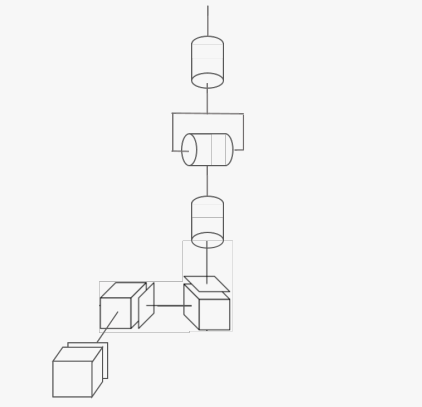
\includegraphics[scale=0.3]{q4_figure.png}
        \centering
    \end{figure}

    (b) Derive $H^1_2$. You can leave sines, cosines, joint values, and link lengths as parameters.
    
    \subsection{Solution for part (a)}

    First we assign coordinate frames 0 through 5 (links 0 through 5). This is done as per the following figure.

    \begin{figure}[h]
        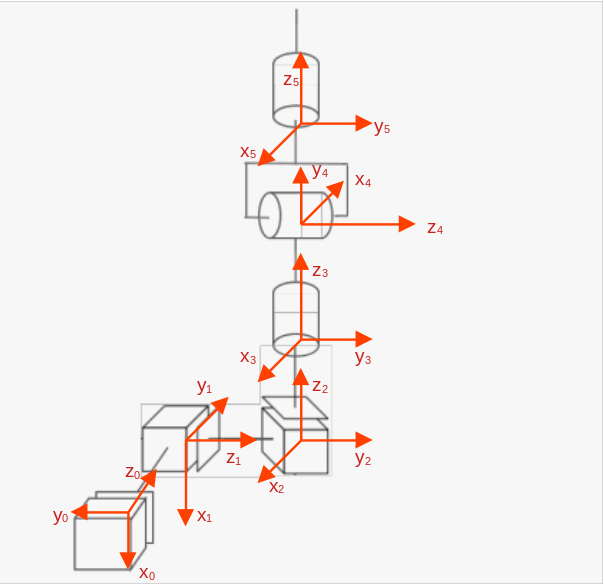
\includegraphics[scale=0.54]{q4_figure_sola.png}
        \centering
    \end{figure}

    Now, we create a table for quantities \(\alpha_i, a_i, \theta_i, d_i\) for links 1 through 6. In this table,
    $d_1$, $d_2$, $d_3$, $\theta_4$, $\theta_5$, $\theta_6$ are variable. However, $l_4$, $l_5$, $l_6$ are fixed (constants).

    \begin{table}[h!]
        \begin{center}
            \begin{tabular}{|c|c|c|c|c|}
            \hline
            Link & $\alpha_i$ & $a_i$ & $\theta_i$ & $d_i$ \\
            \hline
            1 & $90\degree$ & 0 & 0 & $d_1$ \\
            2 & $90\degree$ & 0 & $-90\degree$ & $d_2$\\
            3 & 0 & 0 & 0 & $d_3$\\
            4 & $90\degree$ & 0 & $\theta_4$ & $l_4$\\
            5 & $-90\degree$ & 0 & $\theta_5$ & $l_5$\\
            6 & 0 & 0 & $\theta_6$ & $l_6$\\
            \hline
            \end{tabular}
        \end{center}
    \end{table}

    \subsection{Solution for part (b)}

    We know that \(H^1_2 = A_2\), where $A_2$ is the DH matrix $A_i$ with $i=2$.
    
    \begin{align*}
        H^1_2 = A_2
        &= \begin{bmatrix}
            \cos\theta_2 & -\sin\theta_2 \cos\alpha_2 & \sin\theta_2 \sin\alpha_2 & a_i \cos\theta_2\\
            \sin\theta_2 & \cos\theta_2 \cos\alpha_2 & -\cos\theta_2 \sin\alpha_2 & a_i \sin\theta_2\\
            0 & \sin\alpha_2 & \cos\alpha_2 & d_2\\
            0 & 0 & 0 & 1
        \end{bmatrix}\\
        &= \begin{bmatrix}
            \cos(-90\degree) & -\sin(-90\degree) \cos(90\degree) & \sin(-90\degree) \sin(90\degree) & a_i \cos(-90\degree)\\
            \sin(-90\degree) & \cos(-90\degree) \cos(90\degree) & -\cos(-90\degree) \sin(90\degree) & a_i \sin(-90\degree)\\
            0 & \sin(90\degree) & \cos(90\degree) & d_2\\
            0 & 0 & 0 & 1
        \end{bmatrix}\\
        \alignedbox{H^1_2}{= \begin{bmatrix}0 & 0 & -1 & 0\\ -1 & 0 & 0 & 0\\ 0 & 1 & 0 & d_{2}\\ 0 & 0 & 0 & 1 \end{bmatrix}}
    \end{align*}

\end{homeworkProblem}

\end{document}